\documentclass{beamer}

\usepackage[utf8]{inputenc}
\usepackage[english]{babel}
\usepackage{tikz}
\usepackage{mathtools}
\usepackage{multirow}
\usepackage{anyfontsize}
\graphicspath{{imgs/}}

\newcommand{\NN}{\ensuremath{\mathbb N}}
\newcommand{\ZZ}{\ensuremath{\mathbb Z}}
\newcommand{\QQ}{\ensuremath{\mathbb Q}}
\newcommand{\RR}{\ensuremath{\mathbb R}}
\newcommand{\CC}{\ensuremath{\mathbb C}}
\newcommand{\LL}{\ensuremath{\mathbb L}}
\newcommand{\PP}{\ensuremath{\mathbb P}}

\usetheme{Ilmenau}
\usecolortheme{beaver}

\setbeamerfont{itemize/enumerate subbody}{size=\scriptsize}

\newcommand{\unit}[1]{\ensuremath{\:\text{#1}}}
\newcommand{\pro}{\ensuremath{\unit{\%{}}}}

\expandafter\def\expandafter\insertshorttitle\expandafter{%
  \insertshorttitle\hfill%
  \insertframenumber\,/\,\inserttotalframenumber}

\setbeamertemplate{itemize item}[square]
\setbeamertemplate{itemize subitem}[circle]
\setbeamertemplate{enumerate item}[square]

\title{20 Raspberry Pi's, One Model}

\subtitle{
    Federated Learning On Real Hardware
}
\author[Søren Holm, Asger Schultz, Gustav Moesmand]
{Søren Winkel Holm, Asger Laurits Schultz, Gustav Lang Moesmand}
\institute[DTU]{Technical University of Denmark}
\date{\today}

\begin{document}
\begin{frame}
    \titlepage
\end{frame}

\begin{frame}
    \frametitle{The Presentation}
    \footnotesize
    \tableofcontents
\end{frame}

\section{The Federated Learning Problem}
\begin{frame}
\end{frame}

\begin{frame}
    \frametitle{A Real-Life Setup}
    \noindent
    \parbox[t]{6cm}{
        \begin{itemize}
            \item Most experiments focus only on performance under different hyperparameters
            \item Fail to capture tradeoffs in practical applications
            \item E.g. if few local epochs is better for convergence, is that worth additional overhead?
        \end{itemize}    
    }
    \hfill
    \raisebox{\dimexpr-\height+\baselineskip}{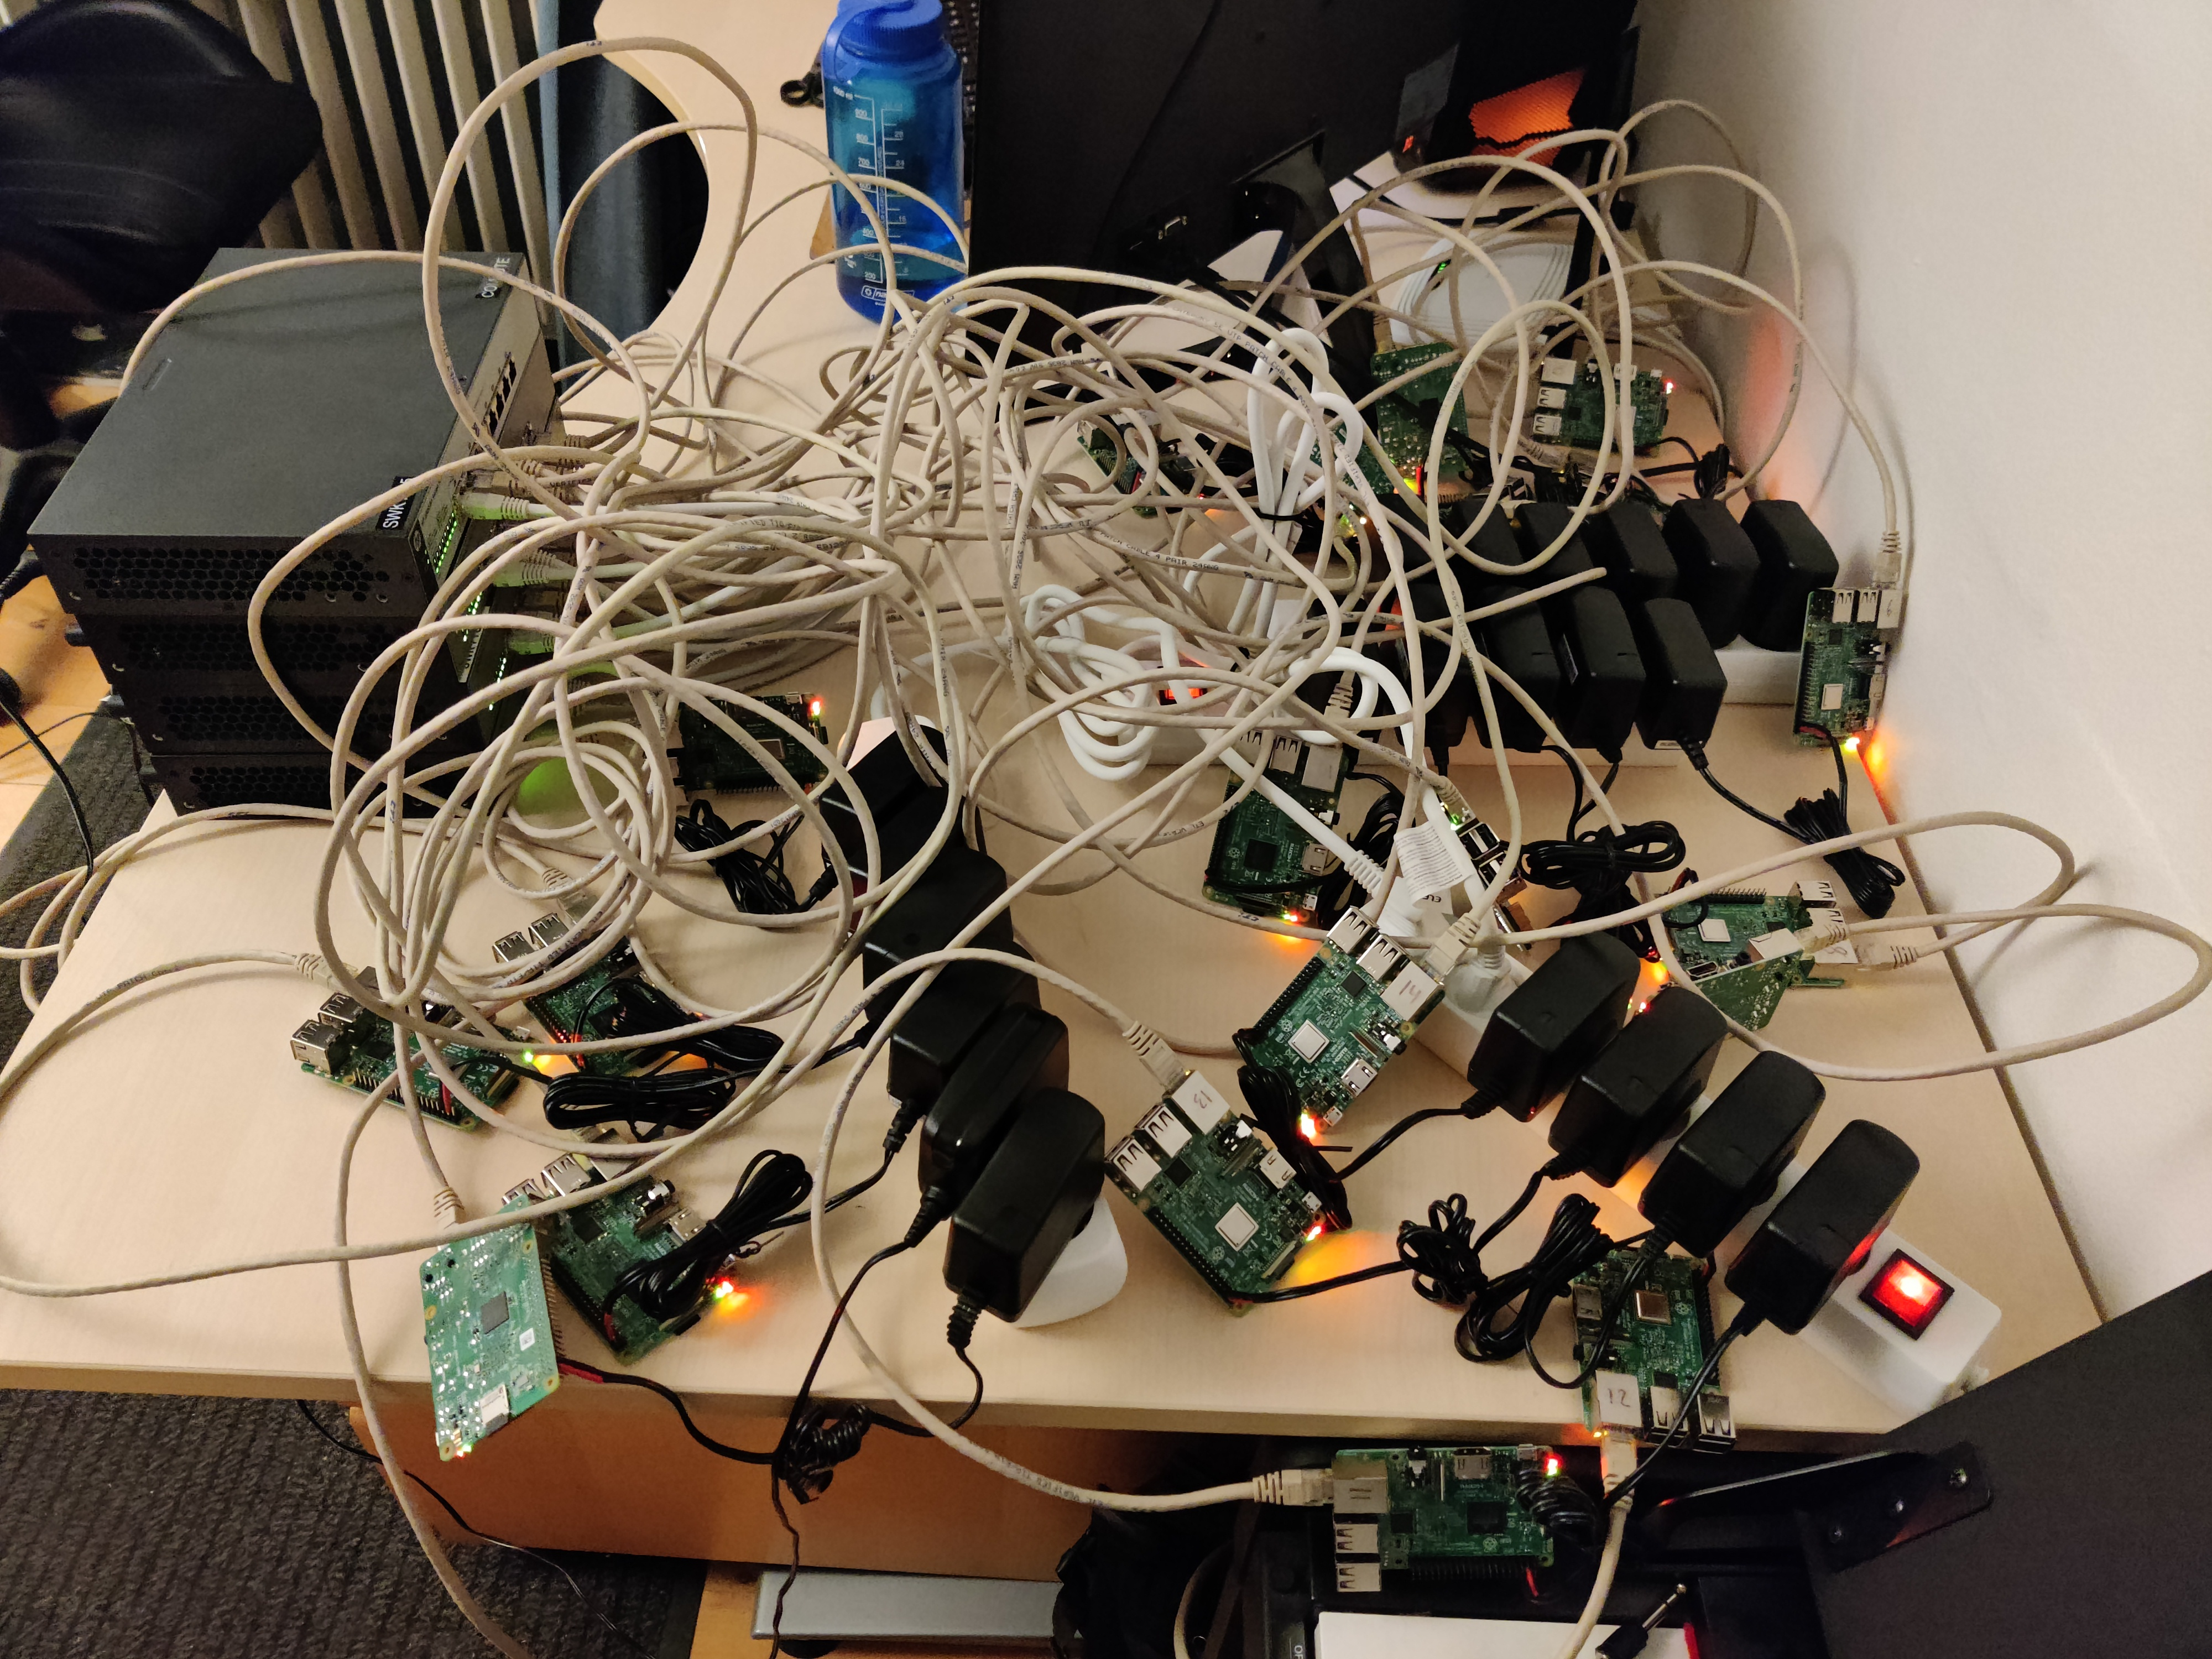
\includegraphics[width=.4\textwidth]{imgs/IMG_20220322_214443}}
\end{frame}

\section{FedAvg on Real Hardware}
\begin{frame}
    \frametitle{FedAvg: The Simple Algorithm [2]}
    \begin{enumerate}
        \item Initialize global model, $\mathcal M_G$
        \item Distribute to $S \le K$ randomly sampled clients
        \item On each client $s$, train local model $\mathcal M_s$ for $E$ epochs
        \item Aggregate models
    \begin{equation*}
        \mathcal M_G \gets \frac{1}{S} \sum_{s=1}^{S} \mathcal M_s
    \end{equation*}
        \item Repeat from step 2 for $L$ communication rounds
    \end{enumerate}
\end{frame}

\begin{frame}
    \frametitle{Parameter Effects}
    \begin{itemize}
        \item Experiments with different parameter choices
        \item $L$ is constant, so larger $E$ increases total number of epochs
    \end{itemize}
    \begin{table}
        \footnotesize
        \centering
        \begin{tabular}{llll}
            \hline
            \multicolumn{4}{c}{Local epochs ($E$)}\\
            1 & 10 & 20 & 40 \\
            \hline
            $48.0 \pm 0.9$ & \textbf{ 52.2 $\pm$ 2.0 } & $37.6 \pm 2.4$ & $22.2 \pm 2.0$ \\
            \multicolumn{4}{c}{Clients samped ($S$)}\\
            5 & 10 & 20 & 40 \\
            \hline
            $35.4 \pm 4.8$ & $37.4 \pm 2.6$ & \textbf{ 38.1 $\pm$ 2.0 } & \textbf{ 38.1 $\pm$ 2.5 } \\
        \end{tabular}
        \caption{Test accuracy in \%\ after 20 communication rounds.}
    \end{table}
\end{frame}

\begin{frame}
    \frametitle{A Practical Case Study}
    \small
    \begin{itemize}
        \item $L=20$ is at very different points for different experiments
        \item Tendency to get worse for too many local epochs
        \item Communication overhead is an important consideration
    \end{itemize}
    \begin{figure}[H]
        \centering
        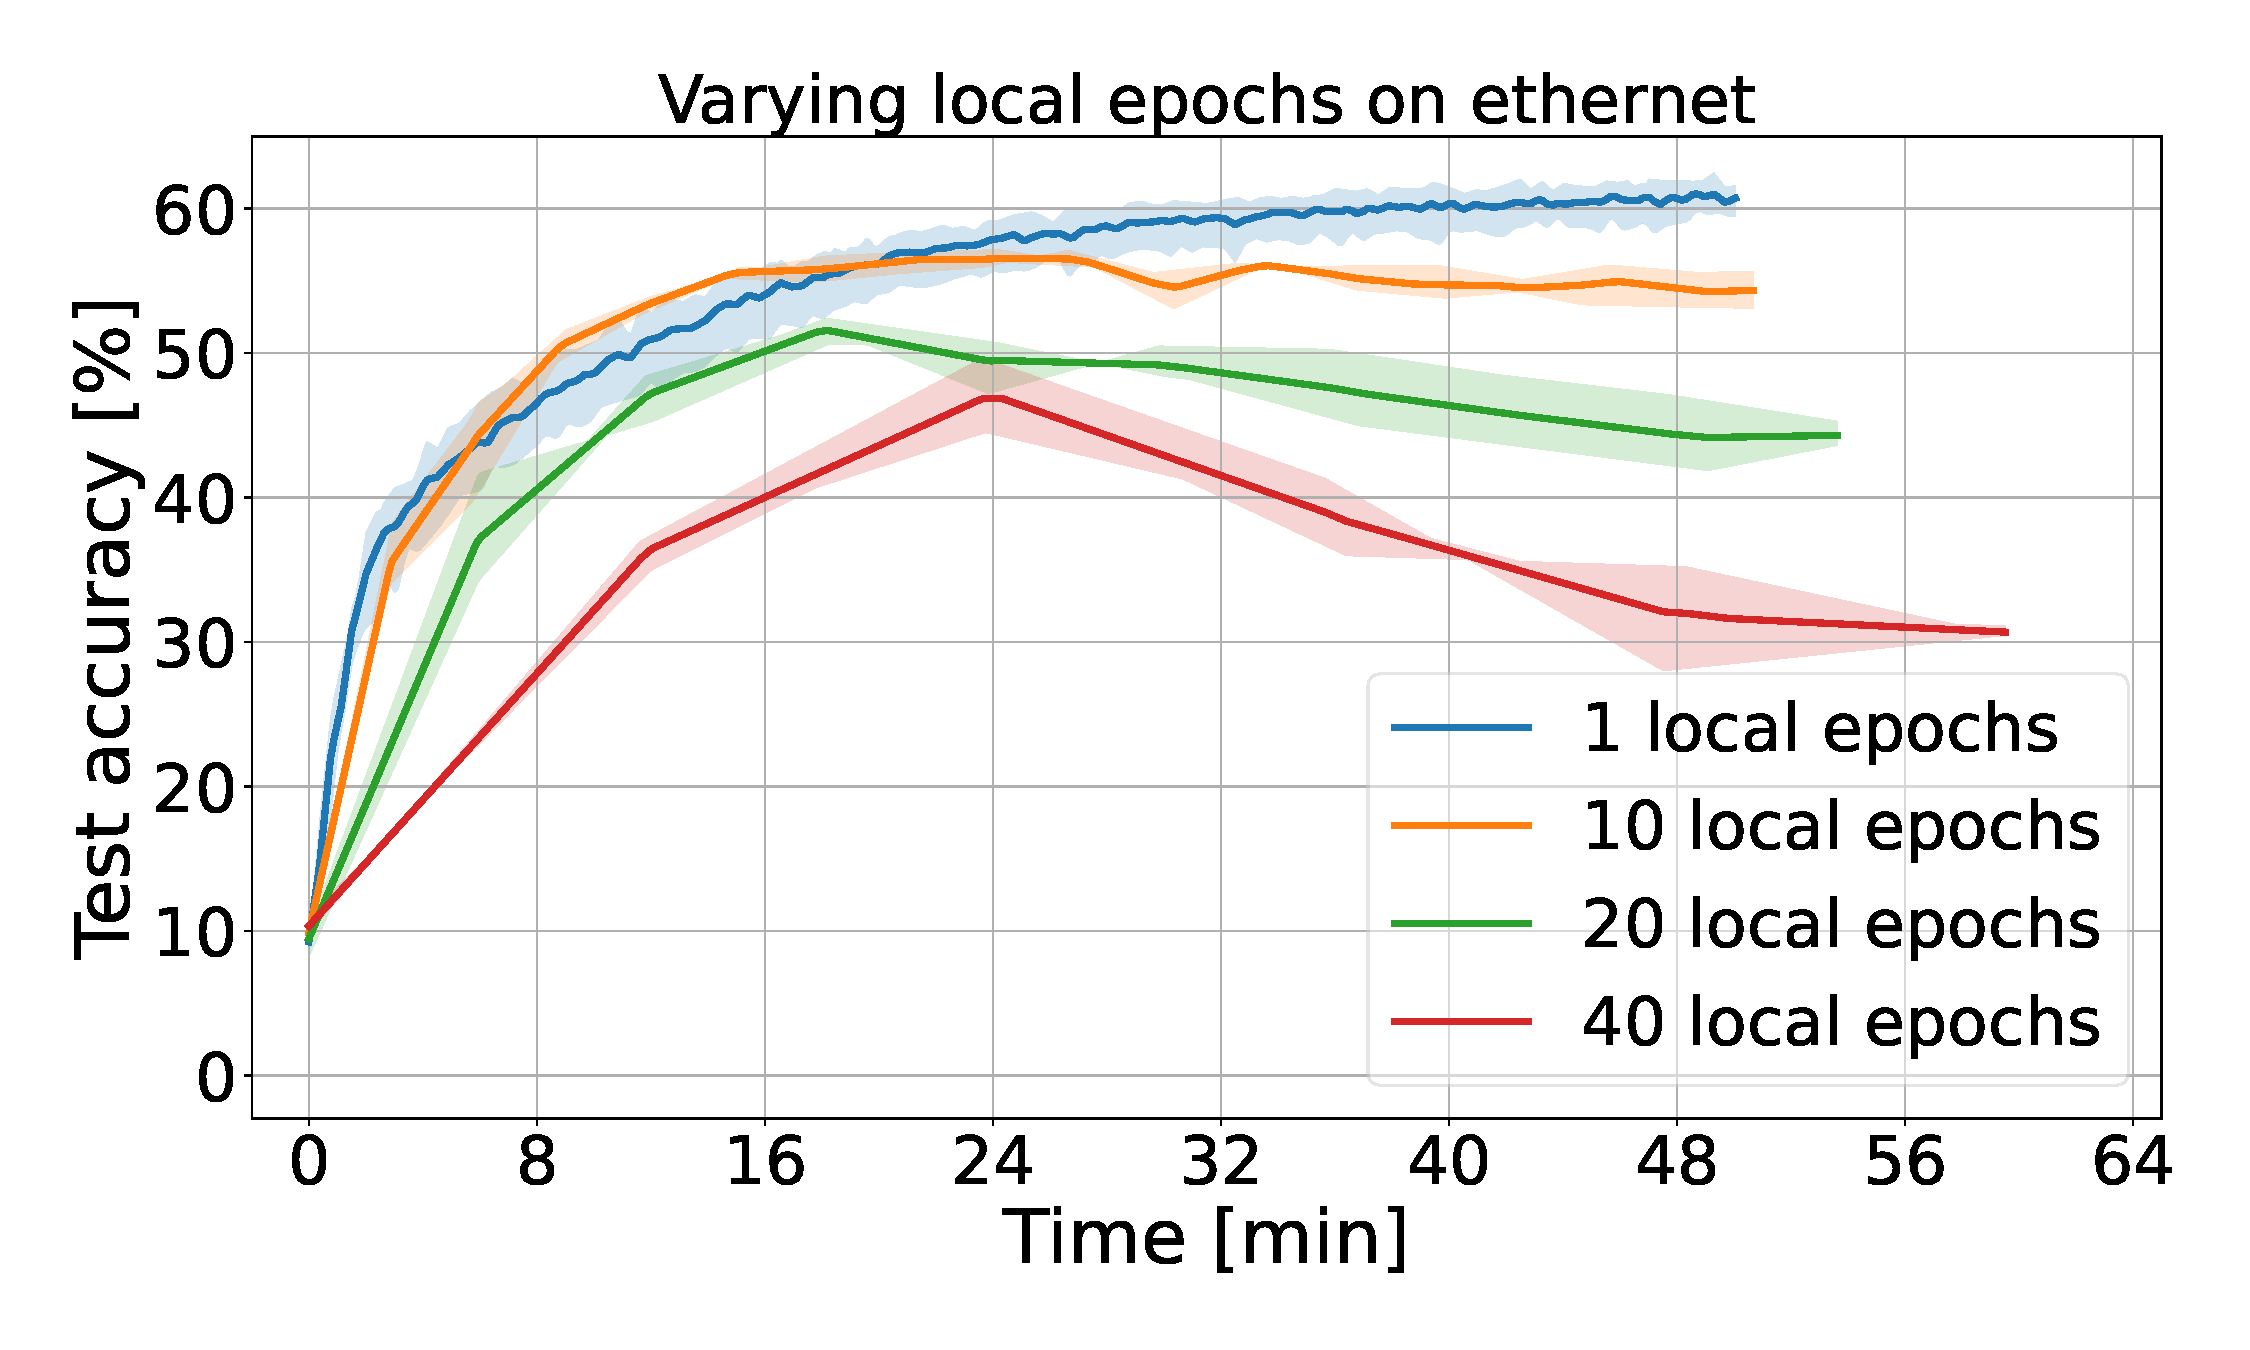
\includegraphics[width=.49\linewidth]{imgs/time_avg_local_epochs_ethernet.pdf}
        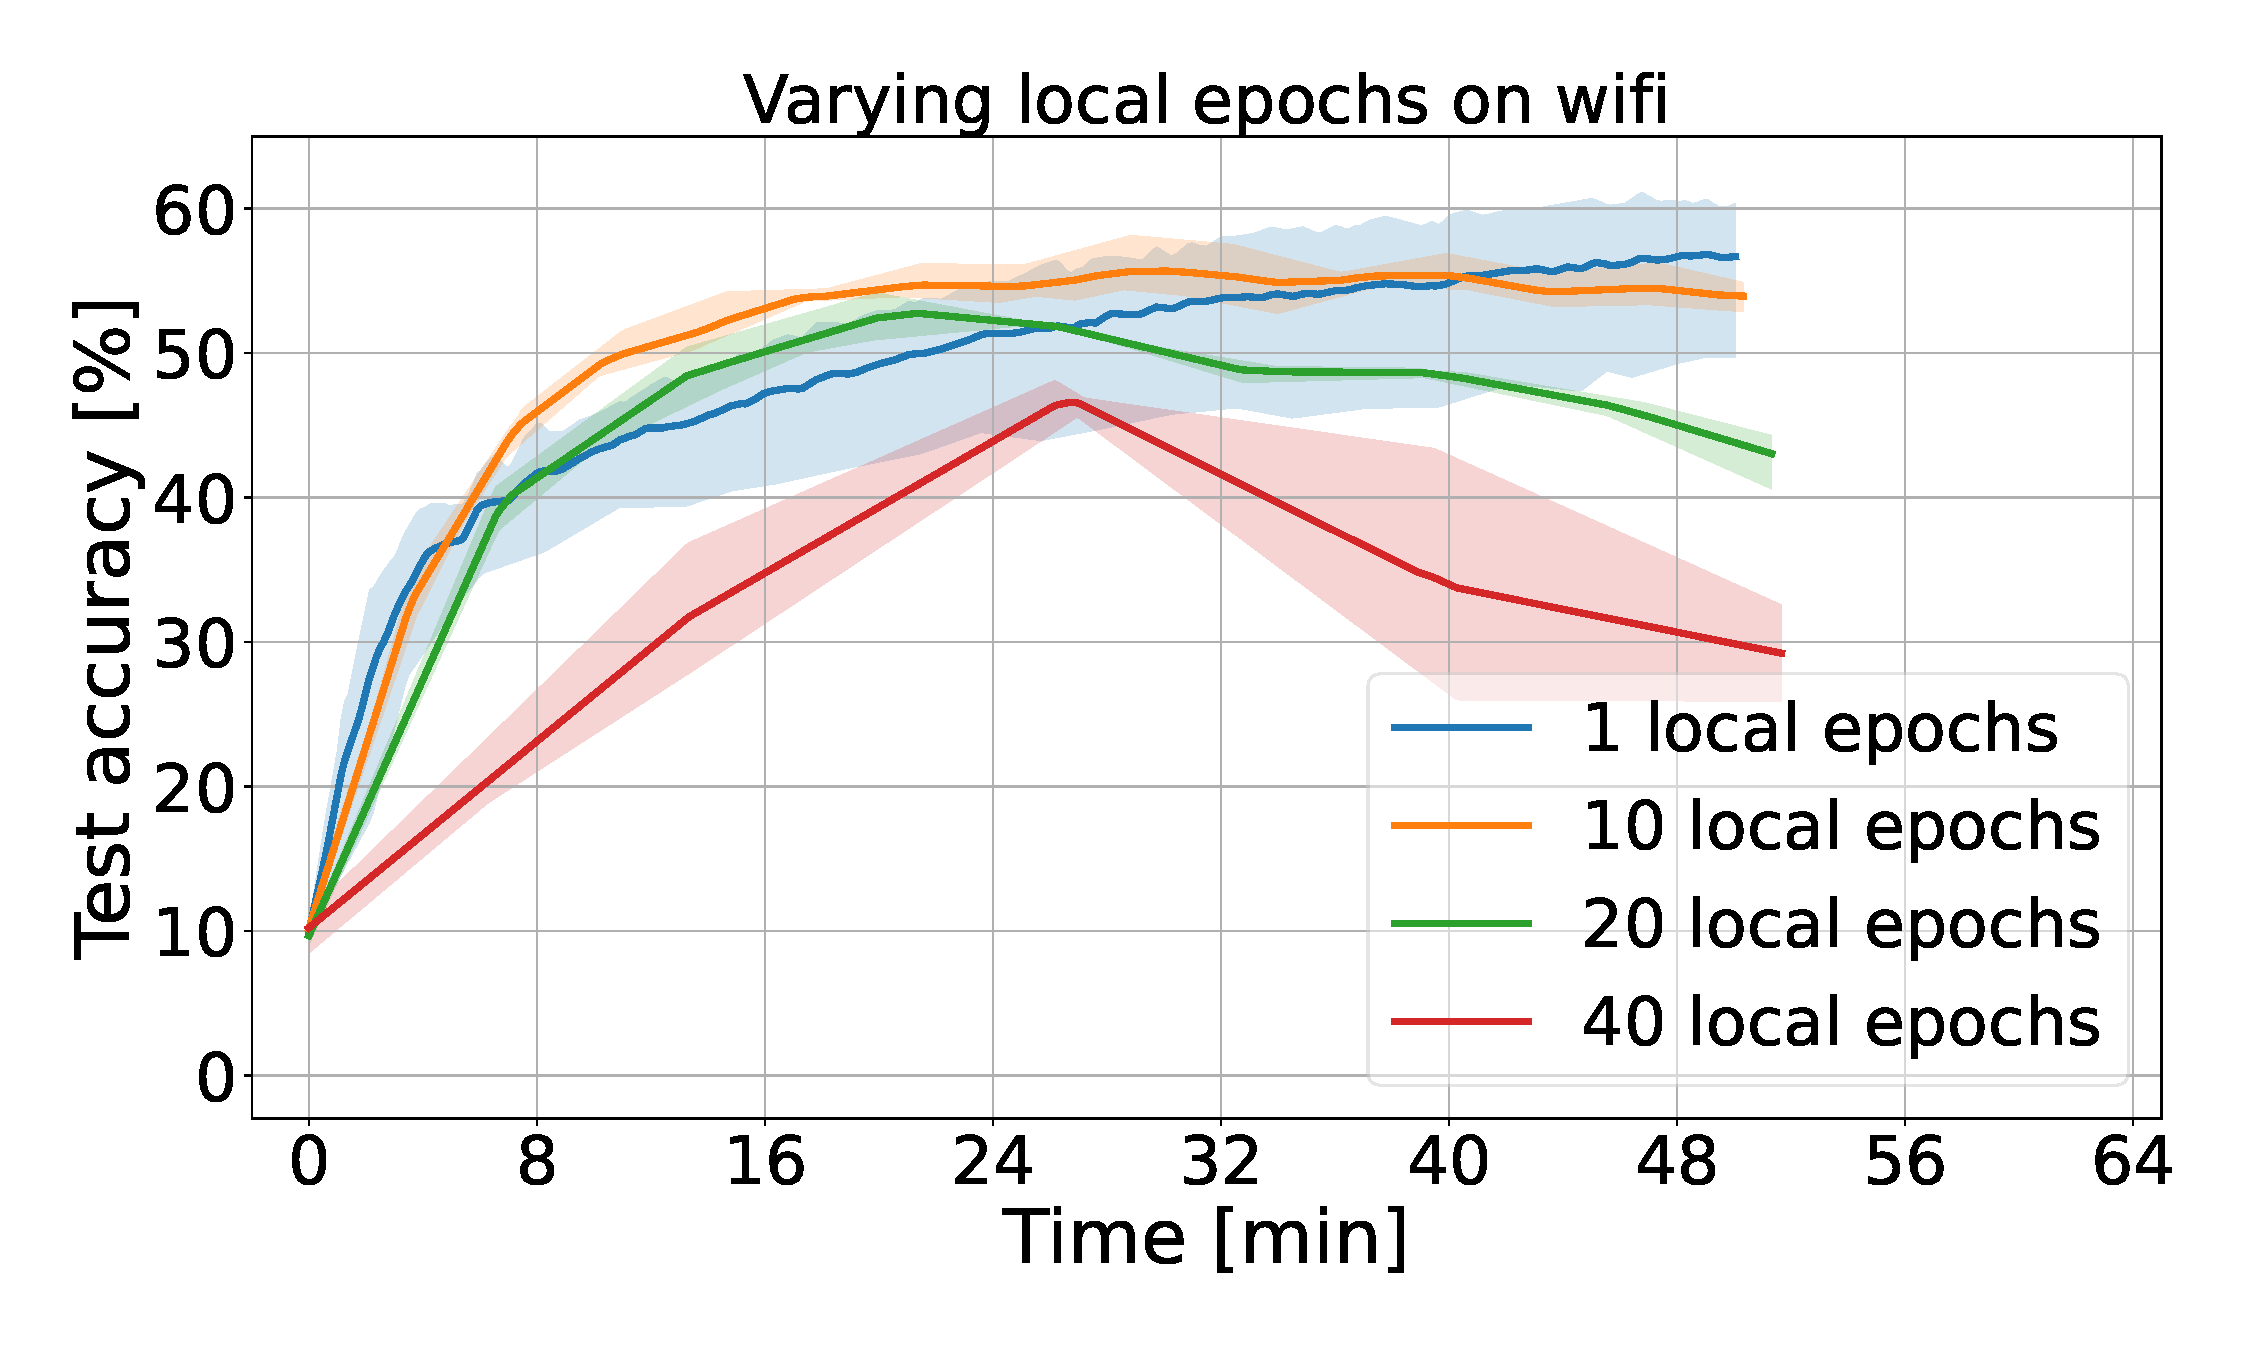
\includegraphics[width=.49\linewidth]{imgs/time_avg_local_epochs_wifi.pdf}
    \end{figure}\noindent
\end{frame}

\begin{frame}
\frametitle{A Practical Case Study, But...}
    \small
    \begin{itemize}
        \item This is just one setup
        \item Simple model with simple dataset
        \item Very little regularization effort
    \end{itemize}
    Our experiment highlights tradeoffs and considerations that in practical applications, but severity and good design choices will vary.
    \begin{figure}[H]
        \centering
        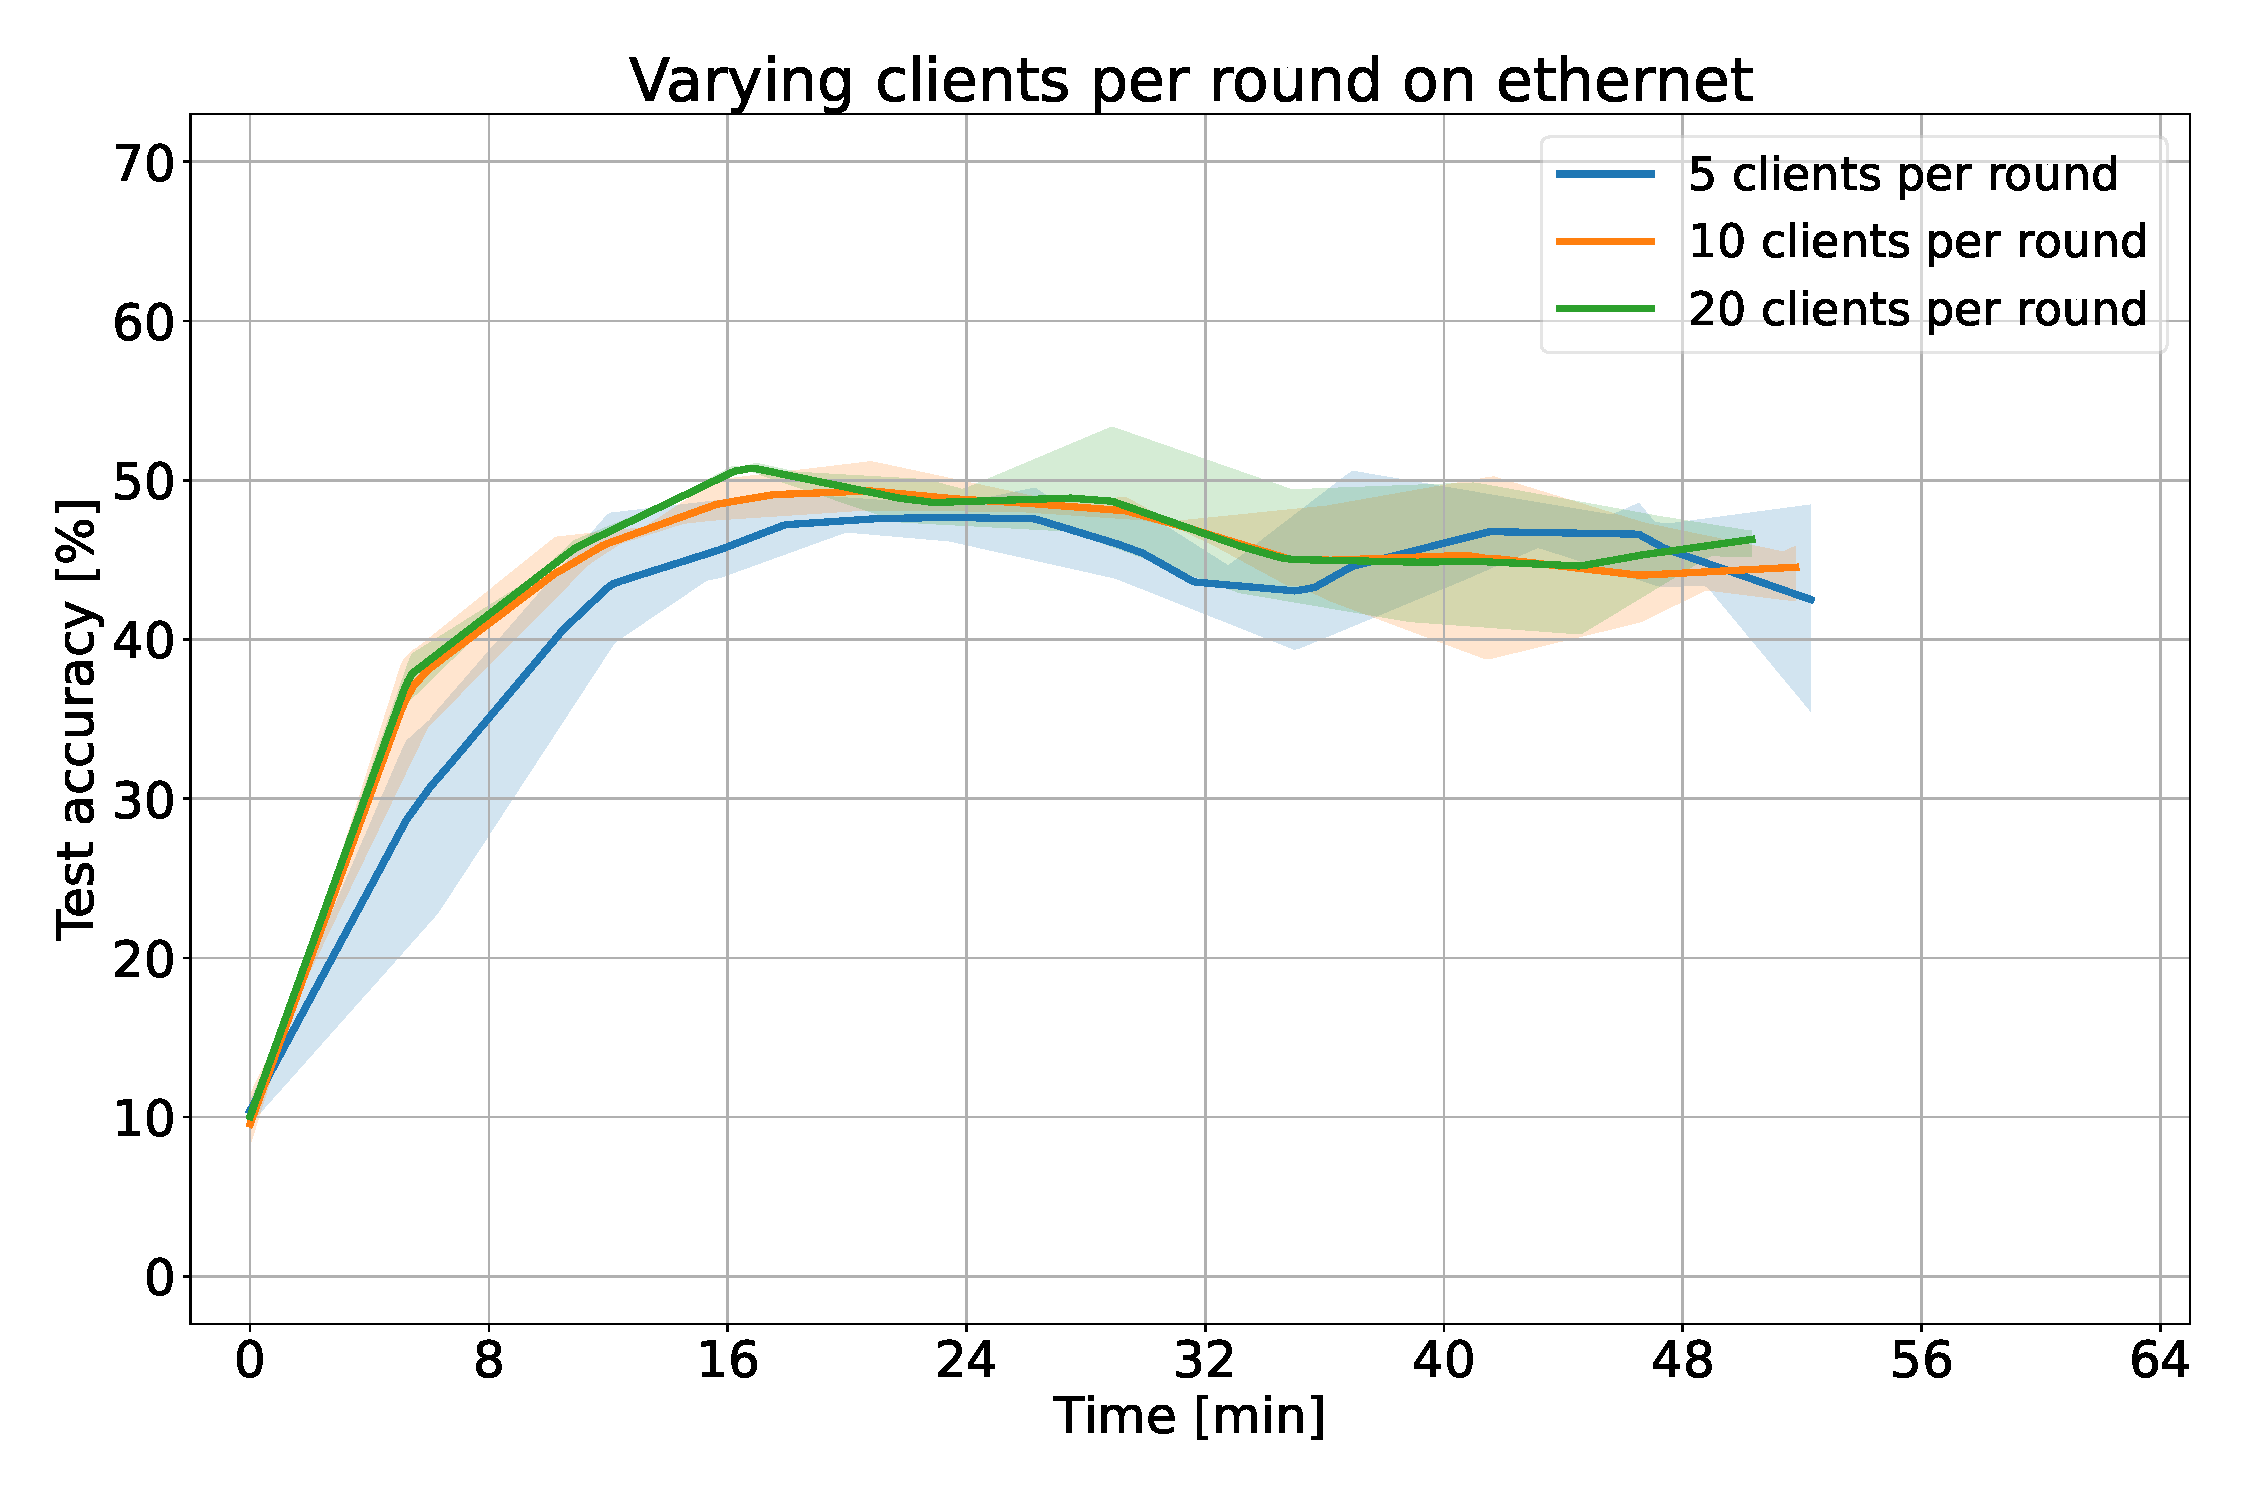
\includegraphics[width=.49\linewidth]{imgs/time_avg_clients_per_round_ethernet.pdf}
        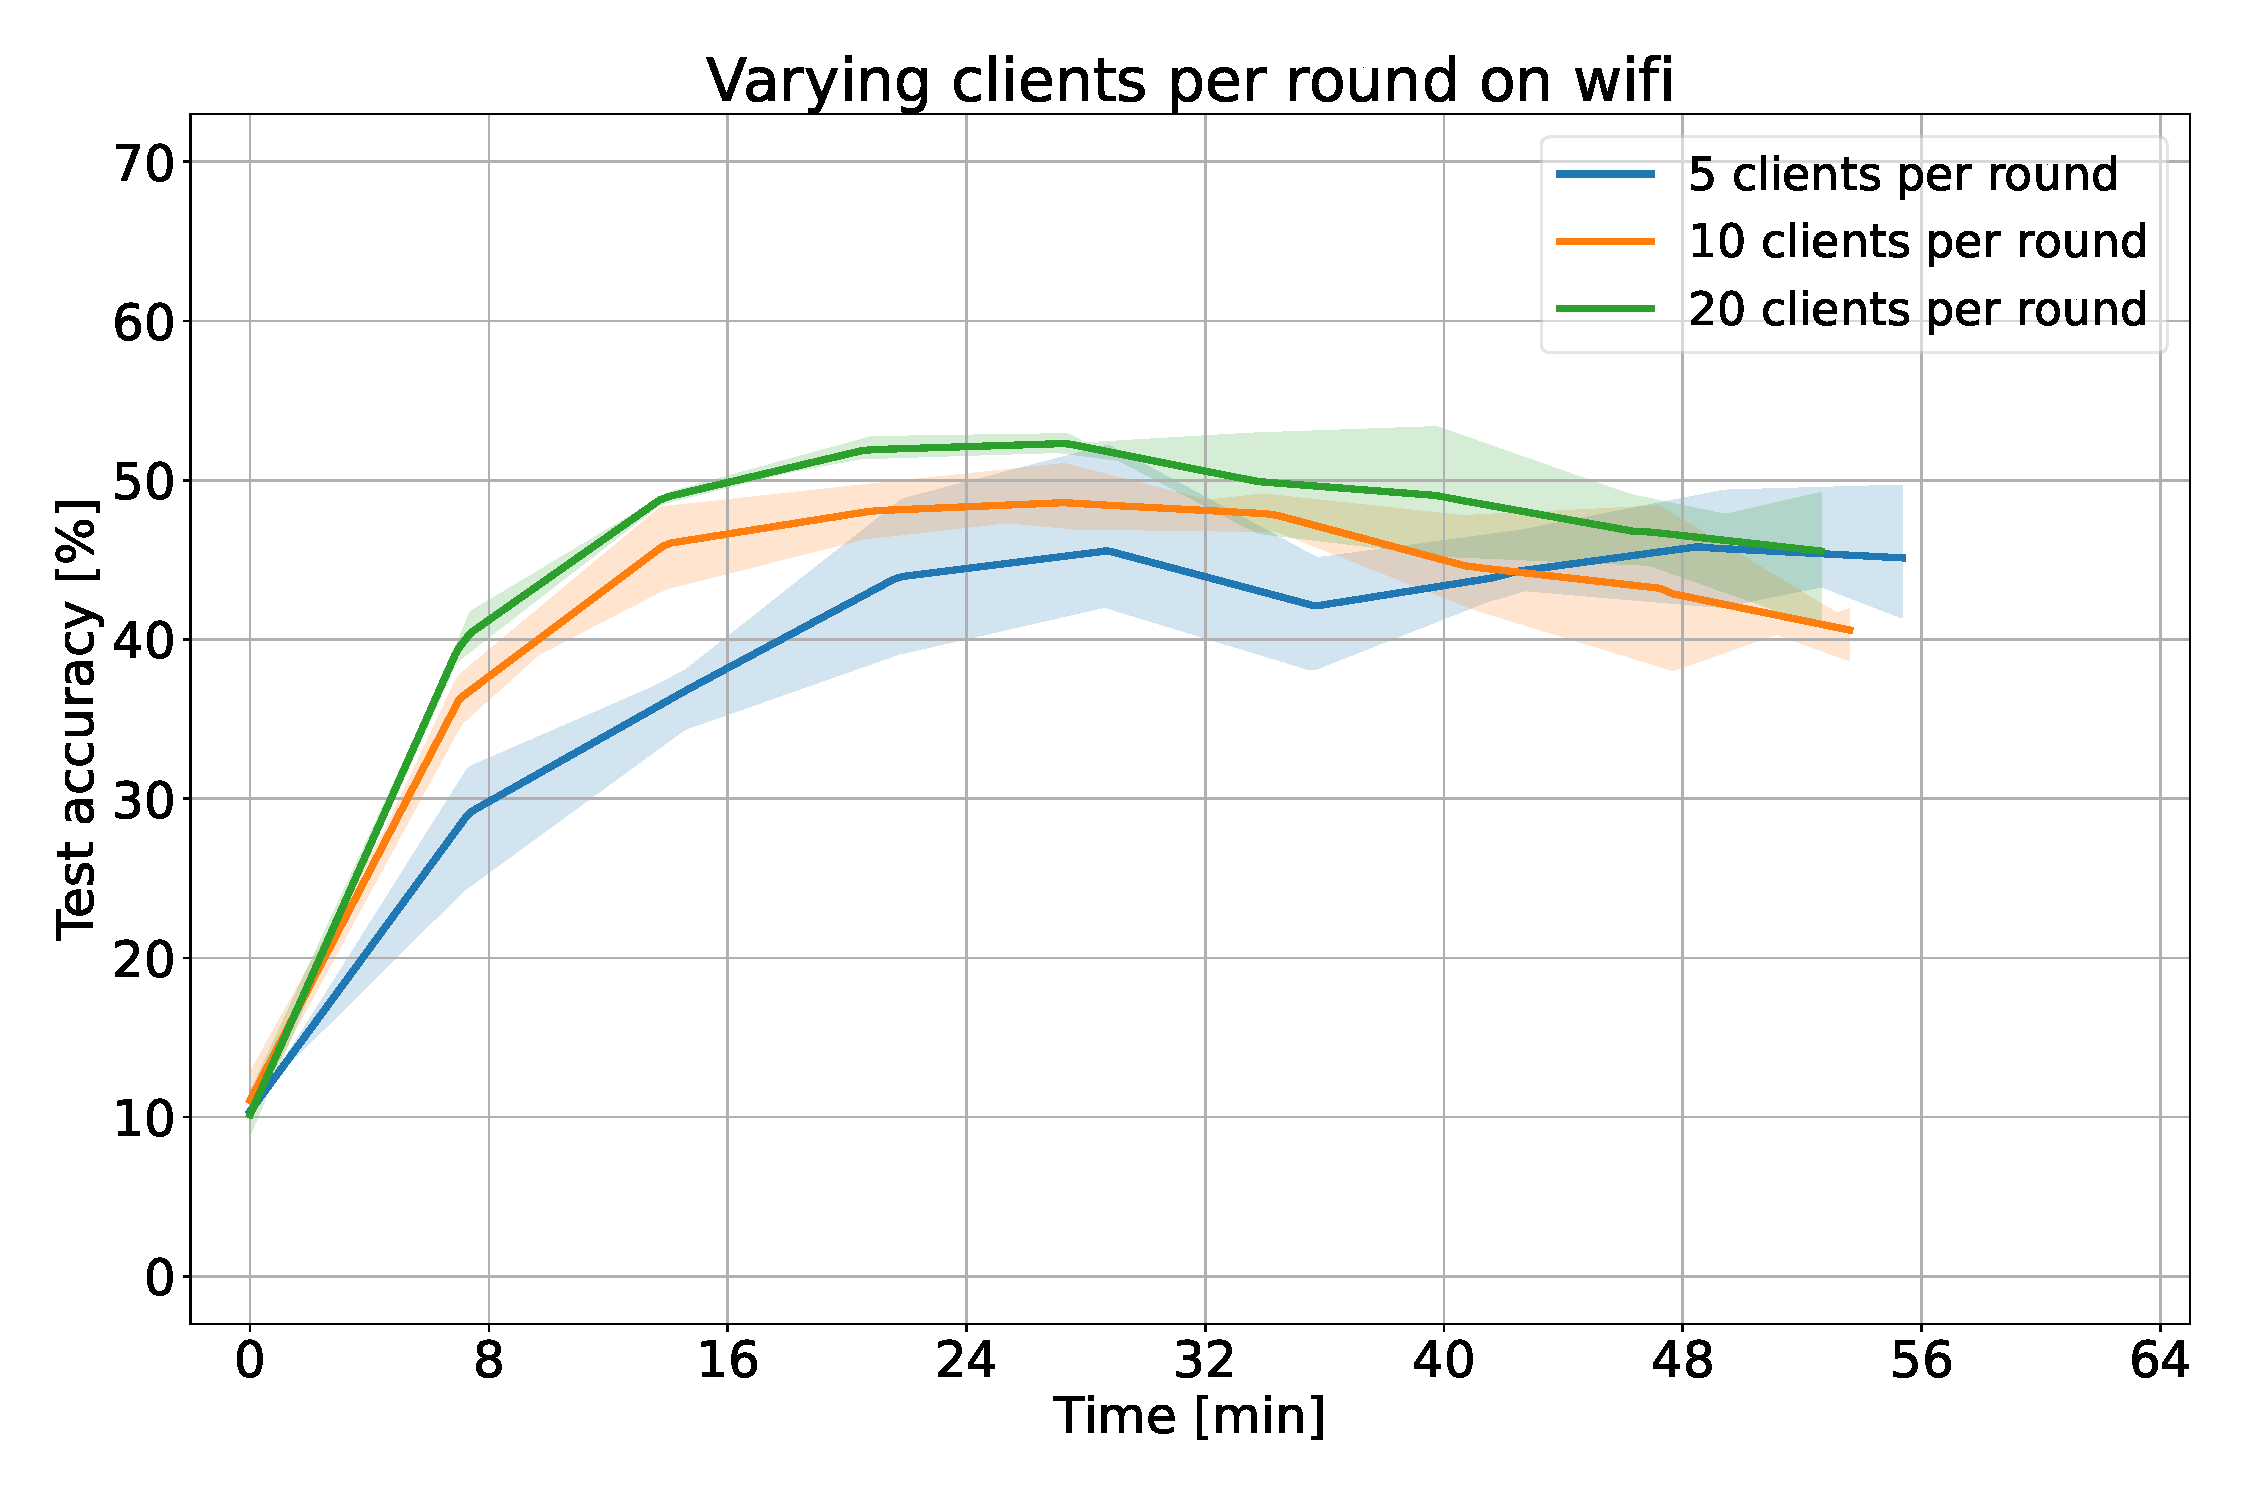
\includegraphics[width=.49\linewidth]{imgs/time_avg_clients_per_round_wifi.pdf}
    \end{figure}\noindent
\end{frame}

\section{Robust Aggregation Using FedDF}
\begin{frame}
    \frametitle{Federated Robustness}
\end{frame}

\begin{frame}
    \frametitle{The FedDF Algorithm}
\end{frame}

\end{document}
